% Options for packages loaded elsewhere
\PassOptionsToPackage{unicode}{hyperref}
\PassOptionsToPackage{hyphens}{url}
%
\documentclass[
]{book}
\usepackage{amsmath,amssymb}
\usepackage{lmodern}
\usepackage{iftex}
\ifPDFTeX
  \usepackage[T1]{fontenc}
  \usepackage[utf8]{inputenc}
  \usepackage{textcomp} % provide euro and other symbols
\else % if luatex or xetex
  \usepackage{unicode-math}
  \defaultfontfeatures{Scale=MatchLowercase}
  \defaultfontfeatures[\rmfamily]{Ligatures=TeX,Scale=1}
\fi
% Use upquote if available, for straight quotes in verbatim environments
\IfFileExists{upquote.sty}{\usepackage{upquote}}{}
\IfFileExists{microtype.sty}{% use microtype if available
  \usepackage[]{microtype}
  \UseMicrotypeSet[protrusion]{basicmath} % disable protrusion for tt fonts
}{}
\makeatletter
\@ifundefined{KOMAClassName}{% if non-KOMA class
  \IfFileExists{parskip.sty}{%
    \usepackage{parskip}
  }{% else
    \setlength{\parindent}{0pt}
    \setlength{\parskip}{6pt plus 2pt minus 1pt}}
}{% if KOMA class
  \KOMAoptions{parskip=half}}
\makeatother
\usepackage{xcolor}
\usepackage{color}
\usepackage{fancyvrb}
\newcommand{\VerbBar}{|}
\newcommand{\VERB}{\Verb[commandchars=\\\{\}]}
\DefineVerbatimEnvironment{Highlighting}{Verbatim}{commandchars=\\\{\}}
% Add ',fontsize=\small' for more characters per line
\usepackage{framed}
\definecolor{shadecolor}{RGB}{248,248,248}
\newenvironment{Shaded}{\begin{snugshade}}{\end{snugshade}}
\newcommand{\AlertTok}[1]{\textcolor[rgb]{0.94,0.16,0.16}{#1}}
\newcommand{\AnnotationTok}[1]{\textcolor[rgb]{0.56,0.35,0.01}{\textbf{\textit{#1}}}}
\newcommand{\AttributeTok}[1]{\textcolor[rgb]{0.77,0.63,0.00}{#1}}
\newcommand{\BaseNTok}[1]{\textcolor[rgb]{0.00,0.00,0.81}{#1}}
\newcommand{\BuiltInTok}[1]{#1}
\newcommand{\CharTok}[1]{\textcolor[rgb]{0.31,0.60,0.02}{#1}}
\newcommand{\CommentTok}[1]{\textcolor[rgb]{0.56,0.35,0.01}{\textit{#1}}}
\newcommand{\CommentVarTok}[1]{\textcolor[rgb]{0.56,0.35,0.01}{\textbf{\textit{#1}}}}
\newcommand{\ConstantTok}[1]{\textcolor[rgb]{0.00,0.00,0.00}{#1}}
\newcommand{\ControlFlowTok}[1]{\textcolor[rgb]{0.13,0.29,0.53}{\textbf{#1}}}
\newcommand{\DataTypeTok}[1]{\textcolor[rgb]{0.13,0.29,0.53}{#1}}
\newcommand{\DecValTok}[1]{\textcolor[rgb]{0.00,0.00,0.81}{#1}}
\newcommand{\DocumentationTok}[1]{\textcolor[rgb]{0.56,0.35,0.01}{\textbf{\textit{#1}}}}
\newcommand{\ErrorTok}[1]{\textcolor[rgb]{0.64,0.00,0.00}{\textbf{#1}}}
\newcommand{\ExtensionTok}[1]{#1}
\newcommand{\FloatTok}[1]{\textcolor[rgb]{0.00,0.00,0.81}{#1}}
\newcommand{\FunctionTok}[1]{\textcolor[rgb]{0.00,0.00,0.00}{#1}}
\newcommand{\ImportTok}[1]{#1}
\newcommand{\InformationTok}[1]{\textcolor[rgb]{0.56,0.35,0.01}{\textbf{\textit{#1}}}}
\newcommand{\KeywordTok}[1]{\textcolor[rgb]{0.13,0.29,0.53}{\textbf{#1}}}
\newcommand{\NormalTok}[1]{#1}
\newcommand{\OperatorTok}[1]{\textcolor[rgb]{0.81,0.36,0.00}{\textbf{#1}}}
\newcommand{\OtherTok}[1]{\textcolor[rgb]{0.56,0.35,0.01}{#1}}
\newcommand{\PreprocessorTok}[1]{\textcolor[rgb]{0.56,0.35,0.01}{\textit{#1}}}
\newcommand{\RegionMarkerTok}[1]{#1}
\newcommand{\SpecialCharTok}[1]{\textcolor[rgb]{0.00,0.00,0.00}{#1}}
\newcommand{\SpecialStringTok}[1]{\textcolor[rgb]{0.31,0.60,0.02}{#1}}
\newcommand{\StringTok}[1]{\textcolor[rgb]{0.31,0.60,0.02}{#1}}
\newcommand{\VariableTok}[1]{\textcolor[rgb]{0.00,0.00,0.00}{#1}}
\newcommand{\VerbatimStringTok}[1]{\textcolor[rgb]{0.31,0.60,0.02}{#1}}
\newcommand{\WarningTok}[1]{\textcolor[rgb]{0.56,0.35,0.01}{\textbf{\textit{#1}}}}
\usepackage{longtable,booktabs,array}
\usepackage{calc} % for calculating minipage widths
% Correct order of tables after \paragraph or \subparagraph
\usepackage{etoolbox}
\makeatletter
\patchcmd\longtable{\par}{\if@noskipsec\mbox{}\fi\par}{}{}
\makeatother
% Allow footnotes in longtable head/foot
\IfFileExists{footnotehyper.sty}{\usepackage{footnotehyper}}{\usepackage{footnote}}
\makesavenoteenv{longtable}
\usepackage{graphicx}
\makeatletter
\def\maxwidth{\ifdim\Gin@nat@width>\linewidth\linewidth\else\Gin@nat@width\fi}
\def\maxheight{\ifdim\Gin@nat@height>\textheight\textheight\else\Gin@nat@height\fi}
\makeatother
% Scale images if necessary, so that they will not overflow the page
% margins by default, and it is still possible to overwrite the defaults
% using explicit options in \includegraphics[width, height, ...]{}
\setkeys{Gin}{width=\maxwidth,height=\maxheight,keepaspectratio}
% Set default figure placement to htbp
\makeatletter
\def\fps@figure{htbp}
\makeatother
\setlength{\emergencystretch}{3em} % prevent overfull lines
\providecommand{\tightlist}{%
  \setlength{\itemsep}{0pt}\setlength{\parskip}{0pt}}
\setcounter{secnumdepth}{5}
\usepackage{booktabs}
\ifLuaTeX
  \usepackage{selnolig}  % disable illegal ligatures
\fi
\usepackage[]{natbib}
\bibliographystyle{apalike}
\IfFileExists{bookmark.sty}{\usepackage{bookmark}}{\usepackage{hyperref}}
\IfFileExists{xurl.sty}{\usepackage{xurl}}{} % add URL line breaks if available
\urlstyle{same} % disable monospaced font for URLs
\hypersetup{
  pdfauthor={Guibor Camargo},
  hidelinks,
  pdfcreator={LaTeX via pandoc}}

\author{Guibor Camargo}
\date{2022-08-01}

\begin{document}

{
\setcounter{tocdepth}{1}
\tableofcontents
}
\hypertarget{ciencia-de-datos-para-politologues}{%
\chapter*{\texorpdfstring{\textbf{Ciencia de datos para politologues}}{Ciencia de datos para politologues}}\label{ciencia-de-datos-para-politologues}}
\addcontentsline{toc}{chapter}{\textbf{Ciencia de datos para politologues}}

\begin{center}\rule{0.5\linewidth}{0.5pt}\end{center}

``\emph{Ciencia de datos para politologues}'' es un libro práctico sobre las principales técnicas de análisis de datos en \textbf{R}. El libro contiene los conceptos y técnicas basicas tanto estadística como computacionales, que son de indispensables conocimiento para estudiante ciencias políticas, relaciones internacionales y/o gestión y desarollo urbanos. Por el lado de la estadística, los contenidos de este libro van desde concepos básicos de estadística descriptiva, hasta el repaso general y práctico de técnicas econométricas de evaluación de impacto y \emph{machine learning}. Por el lado de programación, este libro busca explicar desde el manejo básico de \textbf{R}, hasta algunas técnicas de computación en la nube y la creación de algóritmos de extracción de información y análisis de téxtos (\emph{text-mining}).

\textbf{Un poco sobre mi}

Mi nombre es Guibor, pero por lo general me dicen ``Guibi''. Estudie gestión y desarrollo urbanos en la Facultad de estudios Políticas, Internacionales y Urbanos, de la \emph{Universidad del Rosario} (Colombia), y en esta misma universidad realice mis estudioes de maestría en economía y economía de las políticas públicas. En el día a día trabajo como cíentífico de datos y me gusta mucho tambien trabajar en algunas investigaciones idependientes en diversos temas. \href{https://www.linkedin.com/in/guibor-camargo-salamanca-69bb1981/}{Aqui un poco más de mi peril}.

\textbf{¿Un libro más de ciencia de datos y R? ¿Para qué?}

A lo lagro de mi carrera y en mi ejercicio como investigador, me ha costado mucho encontrar una guía que explique ciertas nociones básicas de estadística y programación para personas que no tengan una formación profesional en máteáticas, estadística y/o economía. Por otro lado, tambien he luchado (y visto muchos luchar) a la hora de trabajar con softwares liecenciados y pagos como Office, ArcGIS, Stata y mucos otros, en los que uno se puede ver atrapado en una de dos sitaciones: O consigues una licencia paga (muy cara) de manera directa o através de la universidad (a través de tramites tediosos que toca anualmente re-hacer), o consigues una licencia pirata exponiendo tu información y tus equipos a cualquier forma de \emph{malware}. Finalmente, si bien hay muy buenos y numerosos recursos en línea, pero estan dispersos, muchas veces solo en ingles, o simplemente son requiren de un buen conocimiento previo de matemáticas, estadística y/o programación e ingeneria de datos para entenderlos, o para entender como se pueden aplicar al mundo del análisis de políticas públicas y sitaciones socio-políticas.

De este modo, este libro busca que cualquier polítologue tenga un muy buen arsenal de herramientas de análisis, y pueda tener (sin importar su conocimiento previo en matemáticas, estadística, programación e ingeneria) una noción básica pero muy robusta de cómo funciona el mundo de la tecnología aplicada a los probelas de ivestigación del día a día. Y finalmente, el libro busca brindar estos conocimientos a través de aprender el uso de \textbf{R}: un lenguaje/sofware de programación oppen source, al alcance de cualquiera con un computaror de manear gratuita y libre, y con una de las comunidades más grande de usuarios en el mundo.

``\url{https://www.youtube.com/watch?v=9i0ElncHGRg}''

\href{mailto:guibor.camargo@urosario.edu.co}{\nolinkurl{guibor.camargo@urosario.edu.co}}

\hypertarget{nociones-buxe1sicas-de-r}{%
\chapter{Nociones básicas de R}\label{nociones-buxe1sicas-de-r}}

Para empezar a utilizar R, es necesario \href{https://cran.r-project.org/bin/windows/base/}{primero descargar el programa}, y preferiblemente tambien \href{https://www.rstudio.com/products/rstudio/download/}{descargar la interfas \emph{Rstudio}}. R es un lenguaje de programación, y \emph{Rstudio} es un entorno en el cuál podemos tener más y vizualización en nuestra interacción con este lenguaje. Un ejemplo útil de esto es la diferencia que hay entre JavaScript y Goolge Chrome: A través de JavaScript y http nos comunicamos con internet, pero a través de Google Chrome intercatuamos con una experienia de usuario con estos protocolos y códigos.

\textbf{Un leguaje de programció orientado a objetos}

\textbf{R} es un \emph{lengaje de progrmación orientado a objetos\textbf{.}} Esto quiere decir, que por ejemplo

\hypertarget{part-anuxe1lisis-espacial}{%
\chapter{(PART*) Análisis espacial}\label{part-anuxe1lisis-espacial}}

\hypertarget{introducicuxf3n-al-anuxe1lisis-epsacial}{%
\chapter{Introducicón al análisis epsacial}\label{introducicuxf3n-al-anuxe1lisis-epsacial}}

Esta guía se base en el curso de \href{https://app.datacamp.com/learn/skill-tracks/spatial-data-with-r?version=1}{Análisis Espacial de Datacamp}, y en algunos recursos disponibles en en linea como recurs1 y recurso 2. Esta guía asume que el lector ya esta famliairizado con:

\begin{itemize}
\item
  Manejo básico de R
\item
  Manejo de las librerias \texttt{dplyr} y \texttt{ggplot2}
\item
  Conceptos básicos de análisis espacial
\end{itemize}

De esta manera, no se hará mucho enfásis en explicar el trasfondo estadístico de algunas de las técnicas aqui explicadas. Los recursos geográficos y tabulares empleados en esta guiá pueden consultarse en el \href{https://drive.google.com/drive/folders/10VeNIEctH2rq7ToQfMKcqeubXemqrKXe?usp=sharing}{este drive}.

\textbf{Acrónicmos}:

\begin{itemize}
\tightlist
\item
  CRS: \emph{Coordinate Reference Systems} (sistemas de coordenadas)
\end{itemize}

\textbf{Librerias previas}

\begin{Shaded}
\begin{Highlighting}[]
\FunctionTok{library}\NormalTok{(dplyr) }\CommentTok{\# Manejo de bases de datos}
\FunctionTok{library}\NormalTok{(tidyr) }\CommentTok{\# Manejo de bases de datos}
\FunctionTok{library}\NormalTok{(ggplot2) }\CommentTok{\# Creación de gráficas}
\FunctionTok{library}\NormalTok{(googledrive) }\CommentTok{\# Conexión con google drive (para descargar datos de pruebas)}
\end{Highlighting}
\end{Shaded}

Antes de inciar, cargeremos la base de homicidios de Bogotá en 2005-2019. Podemos descargarla manualmente del drive de la guia usar el siguietne código.

\begin{Shaded}
\begin{Highlighting}[]
\CommentTok{\# Cargar base de homicidios de dreive}
\NormalTok{\{}\FunctionTok{drive\_download}\NormalTok{(}\FunctionTok{as\_id}\NormalTok{(}\FunctionTok{drive\_ls}\NormalTok{(}\StringTok{"https://drive.google.com/drive/folders/10VeNIEctH2rq7ToQfMKcqeubXemqrKXe?usp=sharing"}\NormalTok{, }\AttributeTok{type =} \StringTok{"csv"}\NormalTok{)}\SpecialCharTok{$}\NormalTok{id), }\AttributeTok{overwrite =}\NormalTok{ T)}
\NormalTok{a01\_homicidios }\OtherTok{\textless{}{-}} \FunctionTok{read.csv}\NormalTok{(}\StringTok{"01\_tabla\_homicidios\_bog\_2005\_2019.csv"}\NormalTok{)}
\FunctionTok{file.remove}\NormalTok{(}\StringTok{"01\_tabla\_homicidios\_bog\_2005\_2019.csv"}\NormalTok{)\}}
\end{Highlighting}
\end{Shaded}

\hypertarget{nociones-buxe1sicas-de-vizualizaciuxf3n}{%
\chapter{Nociones básicas de vizualización}\label{nociones-buxe1sicas-de-vizualizaciuxf3n}}

Hay varias maneras de vizualizar la infromación espacial en \textbf{R}. Sin embargo, partiremos de la manerá mas ``rápida'' y esta es a través de la utilización de ggplot.

\hypertarget{vizualizar-lo-muxe1s-elemental-una-base-de-datos-con-coordenadas}{%
\section{Vizualizar lo más elemental: una base de datos con coordenadas}\label{vizualizar-lo-muxe1s-elemental-una-base-de-datos-con-coordenadas}}

Cuando tenemos una base de puntos, podemos vizualizarla con ggplot2, pero esta vizualización no tiene referencias como un ``mapa base''. Con el comando \texttt{coord\_equal()} podemos hacer que los vertices de las coordeandas sean siempre proporcionales entre sí:

\begin{Shaded}
\begin{Highlighting}[]
\NormalTok{a01\_homicidios }\SpecialCharTok{\%\textgreater{}\%} \FunctionTok{ggplot}\NormalTok{(}\FunctionTok{aes}\NormalTok{(longitude, latitude))}\SpecialCharTok{+}
    \FunctionTok{geom\_point}\NormalTok{()}\SpecialCharTok{+}\FunctionTok{coord\_equal}\NormalTok{()}
\end{Highlighting}
\end{Shaded}

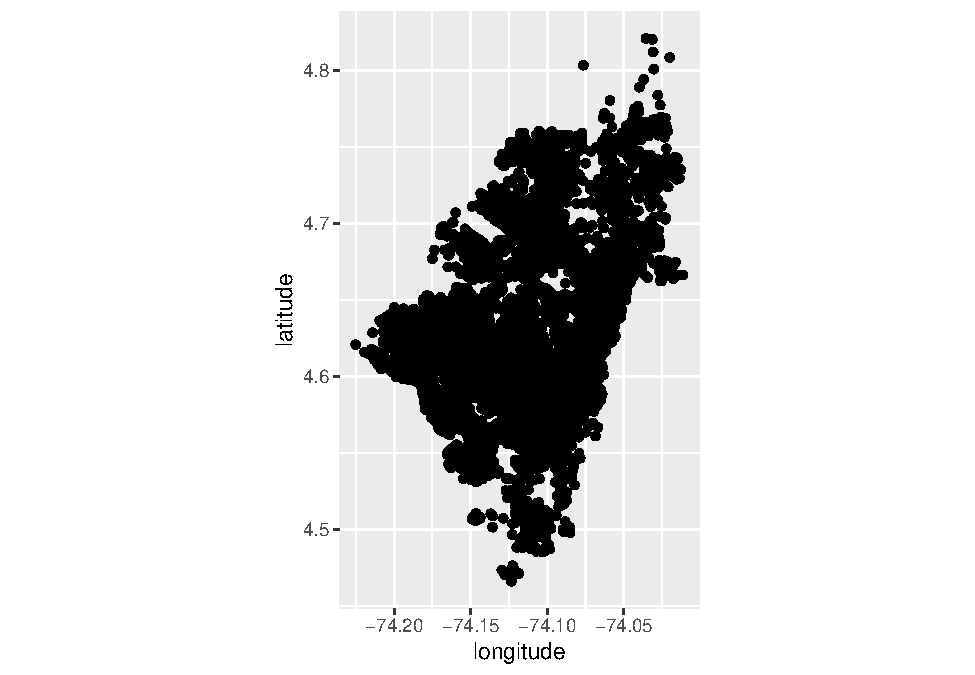
\includegraphics{Data-science-for-political-scientists_files/figure-latex/unnamed-chunk-4-1.pdf}

A pesar de que parece un mecanismo simple hay incluso otros comandos dentro de ggplot2 muy útiles de para vizualizar incuso densidades como \texttt{geom\_bin2d()} y \texttt{geom\_density2d()}

\begin{Shaded}
\begin{Highlighting}[]
\NormalTok{ggpubr}\SpecialCharTok{::}\FunctionTok{ggarrange}\NormalTok{(}
  \CommentTok{\# Lineas de nivlel de densidad}
\NormalTok{   a01\_homicidios }\SpecialCharTok{\%\textgreater{}\%} \FunctionTok{ggplot}\NormalTok{(}\FunctionTok{aes}\NormalTok{(longitude, latitude))}\SpecialCharTok{+}
    \FunctionTok{geom\_density2d}\NormalTok{()}\SpecialCharTok{+}\FunctionTok{coord\_equal}\NormalTok{()}\SpecialCharTok{+}\FunctionTok{labs}\NormalTok{(}\AttributeTok{title =} \StringTok{"\textquotesingle{}geom\_density2d()\textquotesingle{}"}\NormalTok{)}\SpecialCharTok{+}
    \FunctionTok{theme}\NormalTok{(}\AttributeTok{plot.title =} \FunctionTok{element\_text}\NormalTok{(}\AttributeTok{hjust =} \FloatTok{0.5}\NormalTok{)),}
   
\NormalTok{   ggpubr}\SpecialCharTok{::}\FunctionTok{ggarrange}\NormalTok{(}
   
  \CommentTok{\# Densidades simples}
\NormalTok{  a01\_homicidios }\SpecialCharTok{\%\textgreater{}\%} \FunctionTok{ggplot}\NormalTok{(}\FunctionTok{aes}\NormalTok{(longitude, latitude))}\SpecialCharTok{+}
    \FunctionTok{geom\_bin2d}\NormalTok{()}\SpecialCharTok{+}\FunctionTok{coord\_equal}\NormalTok{()}\SpecialCharTok{+}\FunctionTok{labs}\NormalTok{(}\AttributeTok{title =} \StringTok{"\textquotesingle{}geom\_bin2d()\textquotesingle{}"}\NormalTok{)}\SpecialCharTok{+}
    \FunctionTok{theme}\NormalTok{(}\AttributeTok{plot.title =} \FunctionTok{element\_text}\NormalTok{(}\AttributeTok{hjust =} \FloatTok{0.5}\NormalTok{)), }
  
  \CommentTok{\# Densidades lineales}
\NormalTok{  a01\_homicidios }\SpecialCharTok{\%\textgreater{}\%} \FunctionTok{ggplot}\NormalTok{(}\FunctionTok{aes}\NormalTok{(longitude, latitude))}\SpecialCharTok{+}
    \FunctionTok{stat\_density2d}\NormalTok{(}\FunctionTok{aes}\NormalTok{(}\AttributeTok{fill =}\NormalTok{ ..level..),}
                   \AttributeTok{geom =} \StringTok{"polygon"}\NormalTok{, }\AttributeTok{alpha =} \FloatTok{0.3}\NormalTok{)}\SpecialCharTok{+}\FunctionTok{coord\_equal}\NormalTok{()}\SpecialCharTok{+}
    \FunctionTok{labs}\NormalTok{(}\AttributeTok{title =} \StringTok{"\textquotesingle{}stat\_density2d()\textquotesingle{}"}\NormalTok{)}\SpecialCharTok{+}
    \FunctionTok{theme}\NormalTok{(}\AttributeTok{plot.title =} \FunctionTok{element\_text}\NormalTok{(}\AttributeTok{hjust =} \FloatTok{0.5}\NormalTok{)),}
  \AttributeTok{nrow =} \DecValTok{2}\NormalTok{),}
  
  \AttributeTok{nrow =} \DecValTok{1}\NormalTok{)}
\end{Highlighting}
\end{Shaded}

\begin{center}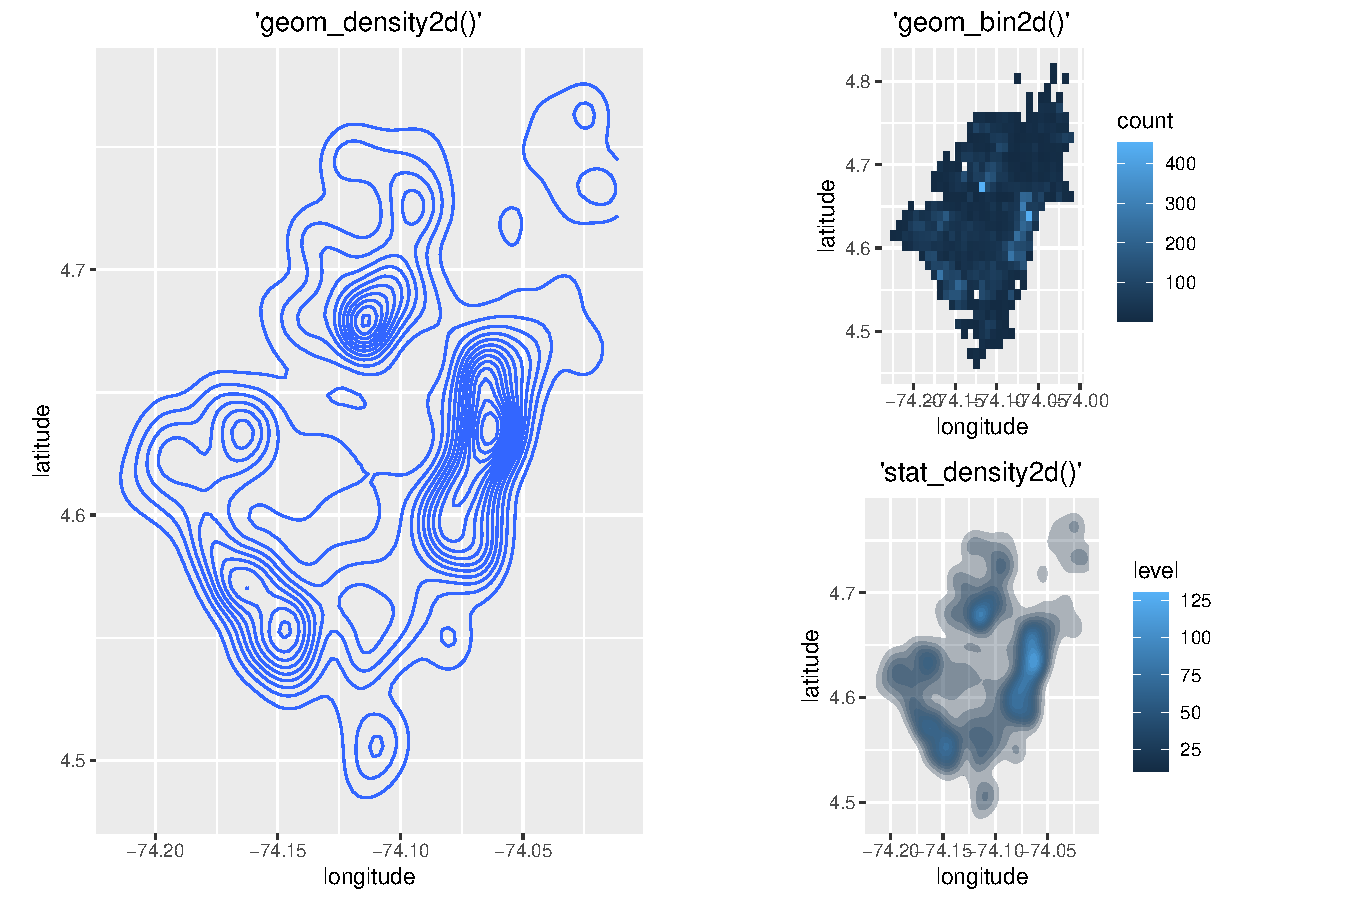
\includegraphics{Data-science-for-political-scientists_files/figure-latex/unnamed-chunk-5-1} \end{center}

\hypertarget{extra-agregando-un-mapa-base-con-ggmap}{%
\section{EXTRA: Agregando un mapa base con `ggmap()'}\label{extra-agregando-un-mapa-base-con-ggmap}}

Auqnue es posible realizar mapas simplemente modificando algunas carácteristicas con ggplot2 de base, hay una libreria \texttt{ggmap()} es una libreria que nos puede ayudar a importar mapas base. Esto no es por lo general necesario, pero en algunos casos puede ser útil para que los lectores del mapa se guien más, o para dalre un acabado más estético a los mapas.

\textbf{LO NO TAN CHEVRE:}

Lo no tan chevre, es que para el uso de esta libreria hay que habilitar el \href{https://mapsplatform.google.com/}{API de Goole Maps}. Los pasos para hbailitar el API son sencillos, pero es necesario registrar una tarjeta de crédito en GCP (Google Cloud Platafform) para que la aplicación no otorgue un \emph{API Key}. No obstane, a pesar de que tenemos que registrar una tarjéta de crédito, dado el bajo consumo que (por lo general) nuestros análisis requiran, no generará cobros. Mas información de esto peude verse con el comando \texttt{help("register\_google")} .

Para agregar una base a estos mapas simples creados desde ggplot, usaremos la libreria \texttt{ggmap()} .

\begin{Shaded}
\begin{Highlighting}[]
\FunctionTok{library}\NormalTok{(ggmap)}
\CommentTok{\# bogota\_mapa\_a \textless{}{-} get\_map(c("lon" = {-}74.10936, "lat" = 4.628712), zoom = 11,}
\CommentTok{\#                        source = "stamen", maptype = "watercolor")}
\CommentTok{\# bogota\_mapa\_b \textless{}{-} get\_map(c("lon" = {-}74.10936, "lat" = 4.628712), zoom = 11,}
\CommentTok{\#                        source = "cloudmade", maptype = 53428)}
\CommentTok{\# }
\CommentTok{\# }
\CommentTok{\# }
\CommentTok{\# }
\CommentTok{\# ggpubr::ggarrange(}
\CommentTok{\#   ggmap(bogota\_mapa\_a,}
\CommentTok{\#         base\_layer = a01\_homicidios \%\textgreater{}\%}
\CommentTok{\#           filter(year == 2019) \%\textgreater{}\%}
\CommentTok{\#           ggplot(aes(longitude, latitude)))+}
\CommentTok{\#     geom\_density2d(color = "red", alpha = 0.7)+}
\CommentTok{\#     labs(title = "Densidad de homicidios Bogotá{-}2019",}
\CommentTok{\#          subtitle = "stamen:watercolor",}
\CommentTok{\#          caption = "Fuente: Policia Metropolitana de Bogotá")+}
\CommentTok{\#     theme(text = element\_text(family = "serif"),}
\CommentTok{\#           plot.title = element\_text(hjust = 0.5),}
\CommentTok{\#           plot.subtitle = element\_text(hjust = 0.5),}
\CommentTok{\#           axis.text = element\_blank(),}
\CommentTok{\#           axis.title = element\_blank()),}
\CommentTok{\# }
\CommentTok{\# ggmap(bogota\_mapa\_b,}
\CommentTok{\#       base\_layer = a01\_homicidios \%\textgreater{}\%}
\CommentTok{\#         filter(year == 2019) \%\textgreater{}\%}
\CommentTok{\#         ggplot(aes(longitude, latitude)))+}
\CommentTok{\#   geom\_density2d(color = "red", alpha = 0.7)+}
\CommentTok{\#   labs(title = "Densidad de homicidios Bogotá{-}2019",}
\CommentTok{\#        subtitle = "stamen:toner",}
\CommentTok{\#        caption = "Fuente: Policia Metropolitana de Bogotá")+}
\CommentTok{\#   theme(text = element\_text(family = "serif"),}
\CommentTok{\#         plot.title = element\_text(hjust = 0.5),}
\CommentTok{\#         plot.subtitle = element\_text(hjust = 0.5),}
\CommentTok{\#         axis.text = element\_blank(),}
\CommentTok{\#         axis.title = element\_blank()),}
\CommentTok{\# nrow = 1)}
\end{Highlighting}
\end{Shaded}

Al igual que casi todo el resto de recursos de R, hay varias \href{https://www.nceas.ucsb.edu/sites/default/files/2020-04/ggmapCheatsheet.pdf}{\emph{cheat-cheats}} y \href{https://journal.r-project.org/archive/2013-1/kahle-wickham.pdf}{guías} en el internet que pocemos consultar para recordar un poco mejor que parámetros podemos emplear en \texttt{source} y \texttt{maptype.}

  \bibliography{book.bib,packages.bib}

\end{document}
